% Created 2024-01-23 Tue 18:46
% Intended LaTeX compiler: xelatex
\documentclass[11pt]{article}
\usepackage{graphicx}
\usepackage{longtable}
\usepackage{wrapfig}
\usepackage{rotating}
\usepackage[normalem]{ulem}
\usepackage{amsmath}
\usepackage{amssymb}
\usepackage{capt-of}
\usepackage{hyperref}
\usepackage{minted}
\usepackage{xeCJK}
\setCJKmainfont{SimSong}
\setCJKmonofont{SimSong}
\let\oldsection\section
\renewcommand{\section}{\clearpage\oldsection}
\author{Chen Chen}
\date{\today}
\title{OCCT OCAF 学习笔记}
\hypersetup{
 pdfauthor={Chen Chen},
 pdftitle={OCCT OCAF 学习笔记},
 pdfkeywords={},
 pdfsubject={},
 pdfcreator={Emacs 29.1 (Org mode 9.7)}, 
 pdflang={English}}
\begin{document}

\maketitle
\tableofcontents

\section{Introduction}
\label{sec:org7dc382d}

\subsection{OCAF Module}
\label{sec:orgd25b56a}

\subsubsection{Overview}
\label{sec:org8c12a91}
Open CASCADE Technology (OCCT) 是一个开源的软件开发平台,用于三维 CAD、CAM、CAE 系统的开发。它提供了广泛的功能,涵盖了几何建模、图形可视化、数据交换和更多方面。

Open CASCADE Application Framework (OCAF) 是 OCCT 中的一个重要模块。OCAF 是一个应用程序框架,用于简化复杂工程图形应用程序的开发。它提供了一种有效的方式来组织、存储、检索和操作复杂的工程数据。OCAF 特别适合于需要处理复杂的装配结构、历史记录、参数化设计等场景的应用程序。
\subsubsection{OCAF 的主要功能}
\label{sec:orgd59d13b}

\begin{itemize}
\item 数据管理
\begin{itemize}
\item OCAF 提供了一套工具来有效地管理和组织数据。
\item 这包括用于创建、管理和修改数据结构的 API
\end{itemize}
\item 历史记录和撤销/重做机制
\begin{itemize}
\item OCAF支持记录用户的操作历史,使得可以方便地实现撤销和重做功能。
\end{itemize}
\item 属性和关系管理
\begin{itemize}
\item OCAF允许开发者为数据元素定义属性(如颜色材料等),并管理数据元素间的关系。
\end{itemize}
\item 事务管理
\begin{itemize}
\item OCAF支持事务管理,这对于保证数据的一致性和完整性非常重要。
\end{itemize}
\item 扩展性
\begin{itemize}
\item OCAF设计灵活,易于扩展,开发者可以根据特定应用需求添加新的功能。
\end{itemize}
\end{itemize}

通过 OCAF,开发者可以更专注于应用的核心功能,而不是底层的数据管理和操作。
\subsubsection{OCAF 的主要 Packages}
\label{sec:orge5ddfef}

下面列出了一些在 OCAF 中常用且重要的 packages:

\begin{itemize}
\item \textbf{TDF (Topological Data Framework)}
\begin{itemize}
\item 用于管理和存储拓扑数据的结构和信息。
\item TDF 提供了一个层次化的数据组织方式,通过 \texttt{Label}, \texttt{Attribute} 等来存储和管理数据
\end{itemize}
\item \textbf{TDocStd (Document Standard)}
\begin{itemize}
\item \texttt{TDocStd} 提供了创建、管理和保存文档的功能
\item 一个文档可以包含一个或多个 TDF 数据结构
\end{itemize}
\item \textbf{XCAF (eXtended CA Framework)}
\begin{itemize}
\item 用于更高级的 CAD 数据处理,如装配结构、颜色和层次信息。
\item XCAF 扩展了 OCAF 的功能,使其能够处理更复杂的 CAD 模型和数据
\end{itemize}
\item \textbf{TNaming (Naming)}
\begin{itemize}
\item 提供了一个命名服务,用于在模型中标识和追踪对象。
\item \texttt{TNaming} 使得在模型变更过程中可以保持对特定对象的引用。
\end{itemize}
\item \textbf{TPrsStd (Presentation Standard)}
\begin{itemize}
\item 用于关联数据模型和其图形表示
\item \texttt{TPrsStd} 允许开发者定义如何将模型数据转换为可视化的图形表示
\end{itemize}
\item \textbf{TDataStd (Data Standard)}
\begin{itemize}
\item 包含了一系列的 Attribute 类型,如字符串、整数、实数、枚举类型等。
\item TDataStd 提供了基础的数据类型,用于存储和处理常规属性。
\end{itemize}
\item \textbf{AppStdL (Application Standard Library)}
\begin{itemize}
\item 提供了一组标准的应用程序功能和服务,如历史管理、撤销/重做机制等。
\end{itemize}
\item \textbf{BinTObj}
\begin{itemize}
\item 用于持久化存储和加载 OCAF 对象的包。
\item 支持二进制格式,适用于大型数据集。
\end{itemize}
\item \textbf{XmlTObj}
\begin{itemize}
\item 类似于 BinTObj,但用于处理基于 XML 的持久化存储和加载。
\end{itemize}
\end{itemize}
\subsection{TDF Package}
\label{sec:org34d64c7}

\subsubsection{Overview}
\label{sec:org94750d2}

TDF (Topology Data Framework) 是 OCAF 的核心组件,用于管理和组织复杂的工程数据(其中拓扑数据是几何建模的基础)。TDF 提供了一个结构化的方式来存储和操作与拓扑相关的信息,如点、线、面、实体等几何元素及其之间的关系。
\subsubsection{TDF 的功能与职责}
\label{sec:orgaf3d645}

\begin{itemize}
\item 数据组织

TDF 提供了一种层次化的数据结构,使得对复杂拓扑数据的管理和访问更加直观灵活。

\item 事务管理

通过 TDF,可以实现对拓扑数据的事务管理,支持撤销/重做操作,保证数据一致性。

\item 属性管理

TDF 允许为拓扑元素附加属性(颜色材料等),并管理这些属性。

\item 关系管理

TDF 支持管理拓扑元素之间的关系,如约束、连接等。

\item 版本控制

TDF 支持数据的版本控制,这对于跟踪数据的历史变更非常有用。

\item 灵活性和扩展性

TDF 设计灵活,易于扩展,可以根据特定的应用需求进行定制。
\end{itemize}
\subsubsection{TDF 的核心类}
\label{sec:org397d009}

\begin{itemize}
\item \texttt{TDF\_Label} class 代表数据结构中的一个节点,可包含多个 sub-Labels 和 Attribute。
\item \texttt{TDF\_Attribute} class 附加在 Label 上的数据单元,用于存储特定类型的信息,如几何数据、颜色、文本等。
\item \texttt{TDF\_Data} class 代表整个数据集合,包含一个或多个 \texttt{TDF\_Label} 树
\item \texttt{TDF\_TagSource} class 用于自动生成唯一的 Tag (标签号)。
\item \texttt{TDF\_RelocationTable} class 在数据复制和粘贴操作中使用,管理 Label 和 Attribute 之间的关系映射。
\end{itemize}
\subsection{TDocStd Package}
\label{sec:orgb77877a}

\subsubsection{Overview}
\label{sec:org5884f4d}
\texttt{TDocStd} 主要用于处理和管理文档(Document),这些文档用于存储和组织复杂的 CAD 数据结构。一个文档通常代表一个工程项目或一个 CAD 模型,它包含了所有相关的数据和信息。 \texttt{TDocStd} 提供了一套工具和接口来创建、管理和存储这些文档。
\subsubsection{TDocStd 的功能与职责}
\label{sec:orgde27626}

\begin{itemize}
\item 文档管理

\texttt{TDocStd} 提供了创建和管理文档的基本机制。文档可以包含多种类型的数据,如几何形状、装配信息、属性等。

\item 文档结构

文档中的数据通过 OCAF 的 \texttt{TDF\_Label} 结构进行组织。每个文档都有一个 root Label, 从 root Label 开始可以创建一个层次化的数据结构。

\item 事务管理

\texttt{TDocStd} 支持事务管理,允许用户对文档进行修改操作,同时支持 Undo/Redo 功能。这对于保持数据的一致性和完整性至关重要。

\item 存储和加载

\texttt{TDocStd} 提供了将文档保存到文件系统和从文件系统加载文档的功能。支持多种格式,包括自定义格式。

\item 版本控制

文档可以支持版本控制,允许跟踪文档的历史变更。

\item 扩展性

\texttt{TDocStd} 的设计允许开发者根据需要扩展和定制文档的功能,以适应特定的应用需求。
\end{itemize}
\subsubsection{TDocStd 与 TDF package 的关系}
\label{sec:org8c927a5}

\begin{itemize}
\item \texttt{TDocStd} 依赖于 \texttt{TDF} 来组织文档内的数据。

每个 \texttt{TDocStd\_Document} 包含一个根 \texttt{TDF\_Label}, 这个 root label 是文档所有数据的起点。通过 root label, 可以访问和操作文档中的所有数据。

\item 在 TDF 基础上,TDocStd 提供了文档级别的管理,如创建/保存/加载文档、事务处理(Undo/Redo)等。
\end{itemize}
\subsubsection{TDocStd 的核心类}
\label{sec:org8a9ff22}

\begin{itemize}
\item \texttt{TDocStd\_Document} class 代表一个文档,是管理和组织 CAD 数据的主要实体。
\item \texttt{TDocStd\_Application} class 处理文档的创建、加载和保存,管理文档集合。
\item \texttt{TDocStd\_Owner} class 作为文档所有者的角色,管理文档的状态和事务。
\end{itemize}
\subsection{XCAF Package (属于 DataExchange Module)}
\label{sec:org898b89d}

\subsubsection{Overview}
\label{sec:orgb267855}

XCAF (eXtended CA Framework) 用于处理更高级别的 CAD 数据,尤其是那些涉及到复杂装配结构的数据。XCAF 提供了一些列工具和接口,用于管理和操作包括颜色、材料、元数据、层级关系等在内的复杂 CAD 模型数据。
\subsubsection{XCAF 主要功能与职责}
\label{sec:org8bd3ef6}

\begin{itemize}
\item 复杂装配结构管理

XCAF 提供了工具来创建和管理复杂的 CAD 装配结构,包括定义装配体、子装配体和零件之间的层级关系。

\item 颜色和图层管理

支持为模型的不同部分指定颜色和图层,帮助改善模型的可视化和组织。

\item 高级属性管理

XCAF 允许为模型元素添加和管理高级属性,如材料属性、PMI(产品和制造信息)、注释和元数据。

\item 形状标识和追踪

提供工具来唯一标识和追踪模型中的形状,尤其在模型的变更或更新过程中,保持对特定形状的引用。

\item 数据交换支持

支持与其他 CAD 系统间的数据交换,特别是在处理 STEP 和 IGES 文件格式时,能够导入和导出中配信息和属性。

\item 扩展性和定制

XCAF 设计灵活,可以根据特定应用需求进行扩展和定制。
\end{itemize}
\subsubsection{XCAF 的核心类}
\label{sec:orgb12b81a}

\begin{itemize}
\item \texttt{XCAFDoc\_ShapeTool} class 用于管理装配结构和形状。
\item \texttt{XCAFDoc\_ColorTool} class 管理颜色属性
\item \texttt{XCAFDoc\_LayerTool} class 管理图层属性
\item \texttt{XCAFDoc\_MaterialTool} class 管理材料属性
\item \texttt{XCAFDoc\_DatumTool}, \texttt{XCAFDoc\_DimTolTool} classes 管理标注和公差。
\item \texttt{XCAFDoc\_AreaStyleTool} class 管理区域样式
\end{itemize}
\subsection{TNaming package}
\label{sec:orgf49d285}

\subsubsection{Overview}
\label{sec:org311606a}

\texttt{TNaming} 提供了命名服务,以便在复杂的 CAD 模型和数据结构中标识和追踪对象。这对于在模型变更过程中保持对特定对象的引用非常重要。
\subsubsection{TNaming 的主要功能与职责}
\label{sec:org26a24c4}

\begin{itemize}
\item 对象标识和追踪

\texttt{TNaming} 允许用户为模型中的对象(如形状、特征等)赋予唯一的名称,从而在整个模型的生命周期中追踪和引用这些对象。

\item 历史追踪

支持记录和跟踪对象随时间的变化。这使得即使在模型被修改或更新后,也能够识别和访问原始对象。

\item 版本控制

\texttt{TNaming} 提供了一种机制来处理模型中对象的版本控制,保证在多次修改和迭代中对象的一致性。

\item 复杂操作支持

对于复杂的操作(如布尔运算、分割、修剪等), \texttt{TNaming} 能够帮助保持对影响的对象的引用,确保数据的准确性和完整性。

\item 与 TDF 协同工作

\texttt{TNaming} 与 \texttt{TDF} 紧密协作,利用 \texttt{TDF\_Label} 和 \texttt{TDF\_Attribute} 来存储和管理命名信息。

\item 撤销/重做机制支持

支持与 OCAF 的撤销/重做机制结合使用,确保在运行这些操作时保持命名信息的一致性。
\end{itemize}
\subsubsection{TNaming 的核心类}
\label{sec:org89ff633}

\begin{itemize}
\item \texttt{TNaming\_NamedShape} class 用于关联形状(Shape)与名称,实现形状的命名和追踪。
\item \texttt{TNaming\_Builder} class 用于构建和修改命名关系
\item \texttt{TNaming\_Tool} class 提供一系列静态方法来操作和查询命名信息
\item \texttt{TNaming\_Naming} class 存储和管理命名操作的历史记录。
\item \texttt{TNaming\_NamingTool} class 提供用于执行复杂命名操作的高级方法
\end{itemize}
\subsection{TPrsStd package}
\label{sec:orgf04b850}

\subsubsection{Overview}
\label{sec:orgfefd789}

\texttt{TPrsStd} package 用于将工程数据(如存储在 OCAF 文档中的数据)与其图形表示相关联。它为开发者提供了一系列工具和接口,以便在图形界面中展示和交互复杂的工程模型。
\subsubsection{TPrsStd 主要功能与职责}
\label{sec:orge8ca565}

\begin{itemize}
\item 图形表示管理

\texttt{TPrsStd} 使得开发者可以将工程数据(如形状、属性等)与其在图形用户界面中的视觉表示相关联。这包括形状的渲染、颜色、纹理等。

\item 交互和选择支持

提供了工具来支持用户与图形表示的交互,包括选择、高亮显示和编辑操作。

\item 属性与视觉同步

确保工程数据的更改能够实时反映在图形表示上,例如当形状发生变化时,其视觉表示也会相应更新。

\item 高级显示功能

支持高级的显示功能,如透明度、阴影和纹理映射,使得工程模型的视觉表示更加逼真和详细。

\item 自定义显示属性

允许开发者定义自己的显示属性和表示方式,以满足特定应用的需求。

\item 与 OCAF 结合使用

\texttt{TPrsStd} 与 OCAF的其他组件(如 \texttt{TDF\_Label}, \texttt{TDF\_Attribute})紧密集成,使得开发者可以方便地管理和同步数据与其图形表示。

\item 支持多种渲染引擎

可以与 OCCT 提供的不同渲染引擎(如OpenGL)协同工作,提供高质量的图形输出。
\end{itemize}
\subsubsection{TPrsStd 的核心类}
\label{sec:orgf07857e}

\begin{itemize}
\item \texttt{TPrsStd\_AISPresentation} class 用于管理工程数据的图形表示,如形状在图形界面中的显示。
\item \texttt{TPrsStd\_AISViewer} class 提供一个视图环境,用于显示和管理多个图形表示。
\item \texttt{TPrsStd\_Presentation} class 作为数据和其图形表示之间的桥梁。
\item \texttt{TPrsStd\_Driver} class 为具体的数据类型提供图形表示的生成和更新逻辑。
\end{itemize}
\subsection{TDataStd package}
\label{sec:orgda5f479}

\subsubsection{Overview}
\label{sec:org88ae92c}

\texttt{TDataStd} 主要提供了一系列标准的数据属性(Attributes),这些属性可以附加到 OCAF 文档中的 Labels 上,用于存储和管理各种类型的数据。
\subsubsection{TDataStd 主要功能与职责}
\label{sec:org8ea6f25}

\begin{itemize}
\item 基本数据类型的管理

\texttt{TDataStd} 提供了用于存储基本数据类型(如字符串、整数、实数、布尔值等)的属性。这些属性用于存储和检索与标签相关联的基本信息。

\item 集合和列表的管理

提供了管理数据集合(如数组、列表)的属性,用于存储多个数据项。

\item 命名和标识符管理

支持为标签分配名称和标识符,方便数据的识别与引用。

\item 枚举和状态管理

提供了用于管理枚举值和状态的属性,可以用于表示有限的选择集或状态机。

\item 文档的元数据管理

支持存储文档级别的元数据,如作者、版本信息、注释等。

\item 与 \texttt{TDF\_Label} 结合使用

\texttt{TDataStd} 的属性与 \texttt{TDF\_Label} 紧密集成,使得数据可以方便地附加到标签上,并在 OCAF 文档的层次化结构中进行管理。
\end{itemize}
\subsubsection{TDataStd 的核心类}
\label{sec:org8cdf33f}

\begin{itemize}
\item \texttt{TDataStd\_Integer} 用于存储和管理整数值
\item \texttt{TDataStd\_Real} 用于存储和管理实数值
\item \texttt{TDataStd\_String} 用于存储和管理字符串
\item \texttt{TDataStd\_UAttribute} 作为用户自定义数据的基类,可以派生出用于存储特定类型数据的类。
\item \texttt{TDataStd\_Name} 用于存储和管理对象的名称
\item \texttt{TDataStd\_Boolean} 用于存储和管理布尔值
\item \texttt{TDataStd\_Enum} 用于存储和管理枚举值
\end{itemize}
\subsection{BinTObj package}
\label{sec:orgf56654d}

\subsection{XmlTObj packages}
\label{sec:org218d636}
\section{开发环境搭建}
\label{sec:org66b83c4}

\subsection{Ubuntu 环境下编译与配置 OCCT 开发环境}
\label{sec:org67b2e43}

\begin{enumerate}
\item 安装依赖

首先安装所有必要的依赖包,通常包括编译器、构建工具和其他库等。

\begin{minted}[]{bash}
  sudo apt-get update
  sudo apt-get install build-essential cmake\
      git libfreetype6-dev libfontconfig1-dev\
      libx11-dev libxext-dev libxt-dev libxmu-dev\
      libgl1-mesa-dev tcl-dev tk-dev
\end{minted}

\item 获取 OCCT 源代码

你可以从 \href{https://dev.opencascade.org/release}{OpenCASCADE} 官网或 \href{https://github.com/Open-Cascade-SAS/OCCT}{GitHub} 上的仓库获取源代码。

\begin{minted}[]{bash}
  mkdir ~/geom
  cd ~/geom
  git clone https://github.com/Open-Cascade-SAS/OCCT.git
\end{minted}

\item 编译与安装 OCCT

\begin{itemize}
\item 使用 CMake 来配置构建系统,创建一个构建目录,在其中运行 cmake

\begin{minted}[]{bash}
    mkdir occt-build
    mkdir occt-install
    cd occt-build
    cmake ../OCCT -DCMAKE_INSTALL_PREFIX=./occt-install
\end{minted}

\item 编译 OCCT 库: \texttt{make -j\$(nproc)}
\item 安装 OCCT 库: \texttt{sudo make install}
\end{itemize}

\item 配置环境变量

设置环境变量以使编译器和连接器能够找到 OCCT 的头文件和共享库。在 \texttt{\textasciitilde{}/.bashrc} 或 \texttt{\textasciitilde{}/.profile} 中添加如下内容

\begin{minted}[]{shell}
  export CASROOT=~/geom/occt-install
  export LD_LIBRARY_PATH=$CASROOT/lib:$LD_LIBRARY_PATH
\end{minted}
\end{enumerate}
\subsection{编写简单的 OCCT 程序}
\label{sec:org8c5b015}

OCCT 安装完成后,我们可以通过编译运行一个简单的 OCCT 示例程序来验证安装。

新建项目目录 \texttt{\textasciitilde{}/hello-occt/}, 新建项目文件 \texttt{CMakeLists.txt} 和 \texttt{main.cpp}. \texttt{CMakeLists.txt} 的内容如下:

\begin{minted}[]{cmake}
cmake_minimum_required(VERSION 3.10)
project(hello-occt)

set(CMAKE_CXX_STANDARD 17)
set(CMAKE_CXX_STANDARD_REQUIRED ON)

find_package(OpenCASCADE REQUIRED)

include_directories(${OpenCASCADE_INCLUDE_DIR})

set(SOURCES main.cpp)
add_executable(${CMAKE_PROJECT_NAME} ${SOURCES})

target_link_libraries(${CMAKE_PROJECT_NAME} ${OpenCASCADE_LIBRARIES})
\end{minted}

\begin{itemize}
\item \texttt{project(hello-occt)} 设置项目的名称
\item \texttt{set(CMAKE\_CXX\_STANDARD 17)} 指定 C++ 标准
\item \texttt{find\_package(OpenCASCADE REQUIRED)} 查找并加载 OCCT 库
\item \texttt{include\_directories(\$\{OpenCASCADE\_INCLUDE\_DIR\})} 添加 OCCT 头文件的路径
\item \texttt{set(SOURCES ...)} 定义了项目的源文件
\item \texttt{add\_executable(\$\{CMAKE\_PROJECT\_NAME\} \$\{SOURCES\})} 创建一个可执行文件
\item \texttt{target\_link\_libraries(\$\{CMAKE\_PROJECT\_NAME\} \$\{OpenCASCADE\_LIBRARIES\})} 链接 OCCT 库
\end{itemize}

下面的验证程序,创建一个简单的长方体,然后获取其 Topo Shape。源代码文件 \texttt{main.cpp} 如下

\begin{minted}[]{cpp}
#include <iostream>
#include <BRepPrimAPI_MakeBox.hxx>
#include <TopoDS_Shape.hxx>

int main() {
  BRepPrimAPI_MakeBox box(1., 2., 3.);
  const TopoDS_Shape& shape = box.Shape();
  std::cout << "Hello OCCT" << std::endl;
  return 0;
}
\end{minted}

按照如下的方式编译并执行程序

\begin{minted}[]{bash}
mkdir build
cd build
cmake ..
cmake --build .
./hello-occt
\end{minted}

程序执行成功的话,会打印 \texttt{Hello OCCT} 。
下面穿插介绍一下涉及的 OCCT clases。
\subsection{相关的 OCCT 类}
\label{sec:org3659e94}

\subsubsection{\texttt{BRepPrimAPI\_MakeBox} class}
\label{sec:orge9756c2}

\texttt{BRepPrimAPI\_MakeBox} 这个类是 OCCT 中 BRep 建模的一部分,用于创建三维的长方体(盒子)。长方体可以通过指定宽度、高度和深度来定义,也可以通过其他方式如两个对角点或中心点和尺寸来定义。它的一些关键接口有:

\begin{itemize}
\item \texttt{BRepPrimAPI\_MakeBox(gp\_Pnt\& P, Standard\_Real dx, Standard\_Real dy, Standard\_Real dz)}: 以点 \texttt{P} 作为长方体的一个角,并指定长方体在三个方向上的尺寸 \texttt{(dx, dy, dz)} 来创建长方体。
\item \texttt{BRepPrimAPI\_MakeBox(Standard\_Real dx, Standard\_Real dy, Standard\_Real dz)}: 创建一个以原点为一个角的长方体,尺寸为 \texttt{(dx, dy, dz)}
\item \texttt{BRepPrimAPI\_MakeBox(gp\_Pnt\& P1, gp\_Pnt\& P2)}: 以两个对角点 \texttt{P1} 和 \texttt{P2} 来创建长方体。
\item \texttt{BRepPrimAPI\_MakeBox(gp\_Ax2\& Axes, Standard\_Real dx, Standard\_Real dy, Standard\_Real dz)}: 以 \texttt{Axes} 定义的坐标系为参考,创建尺寸为 \texttt{(dx, dy, dz)} 的长方体
\item \texttt{Shape()} 方法可以获取生成的长方体形状 (\texttt{TopoDS\_Shape} 类型)。
\end{itemize}
\subsubsection{\texttt{TopoDS\_Shape} class}
\label{sec:orga65e88b}

\texttt{TopoDS\_Shape} 是 OCCT 的一个核心类,用于表示和操作几何形状。 \texttt{TopoDS\_Shape} 是所有几何形状的基类,包括点、线、面、实体等,它为各种几何实体提供了一种通用的访问和操作方式。它的一些重要的接口有:

\begin{itemize}
\item \texttt{IsNull()}: 检查形状是否为空(引用为空)。
\item \texttt{IsEmpty()}: 检查形状是否为空或没有几何信息。
\item \texttt{TShape()}: 返回 Shape 的一个 handle。
\item \texttt{Orientation()}, \texttt{Orientation(TopAbs\_Orientation)}: 获取和设置 Shape 的方向
\item \texttt{Location()}, \texttt{Location(const TopLoc\_Location\&)}: 获取和设置 Shape 的局部坐标系(local coordinate system)
\item \texttt{Located(const TopLoc\_Location\&)}: 获取一个当前 Shape 在新位置处的副本。
\item \texttt{Move(const TopLoc\_Location\&)}: 移动 Shape 的位置。
\item \texttt{Moved(const TopLoc\_Location\&)}: 获取一个当前 Shape 移动后的副本
\item \texttt{Reverse()}: 反转形状的方向 (orientation)
\item \texttt{Reversed()}: 获取一个当前 Shape 反转方向后的副本
\item \texttt{ShapeType()}: 获取 Shape 的类型,如 \texttt{TopAbs\_VERTEX}, \texttt{TopAbs\_EDGE}, \texttt{TopAbs\_FACE} 等。
\end{itemize}
\section{如何基于 OCAF 构建应用程序 (draft)}
\label{sec:org411ef92}

设计一个基于 OCAF 的应用,就是定义一个 Application class,它需要集成 \texttt{TDocStd\_Application} 类。概念上,Application class 中定义了整体的 data model 和 App behavior(即 data model 支持的操作)。App 的 data model 是基于 \texttt{TDocStd\_Document} 实现的。

实现一个基于 OCAF 的应用程序,步骤大致如下:

\begin{enumerate}
\item 定义一个继承自 \texttt{TDocStd\_Application} 的 App 类。为其,创建一个 \texttt{Resource\_Manager} 并指定其文档格式
\begin{itemize}
\item \texttt{TDocStd\_Application} 是 abstract class,为啥能直接 \texttt{new} 呢
\item 文档中的示例太老旧了。看了代码,目前还没明白 Resource 和 Format 的底层机制
\item Resource 是配置文件吗?其中定义了每种格式的读写机制,以及插件?
\begin{itemize}
\item 这里的插件具体又是什么?
\end{itemize}
\item 为了加载读写机制(共享库?)需要设置两个环境变量 \texttt{CSF\_PluginDefaults} 和 \texttt{CSF\_ResourcesDefault}, 两个变量分别指定 plugin file 和 resource file 的目录。
\end{itemize}
\item 定义 App class 的 data model。通过组织 Document 的 Label 和 Attribute 的层次结构,来构建 data model。你可以创建自定义的 Attribute 类型。
\item 实现一些 App Commands。通过这些 Commands 用户可以创建或修改 data model。Data model 中可以包含 persistent references 用于关联任何数据,如 Geom-Elements 或 Documents。其中 OCAF 提供了 Save/Open documents, Undo/Redo commands 等功能。
\item 对 Document 和 View 进行关联
\item 将整个 App 继承到其他的 GUI 框架中,如 QT, MFC 等。
\end{enumerate}
\subsection{Resource File}
\label{sec:org223e2df}

Resource file 定义了各种文档格式 formats (type + extension),和各种数据类型的读写驱动 (drivers)。

每种驱动都有一个唯一的 GUID 标识,比如下面五个常见驱动:

\begin{itemize}
\item the schema driver (ad696002-5b34-11d1-b5ba-00a0c9064368)
\item the document storage driver (ad696000-5b34-11d1-b5ba-00a0c9064368)
\item the document retrieval driver (ad696001-5b34-11d1-b5ba-00a0c9064368)
\item the attribute storage driver (47b0b826-d931-11d1-b5da-00a0c9064368)
\item the attribute retrieval driver (47b0b827-d931-11d1-b5da-00a0c9064368)
\end{itemize}

而这些 drivers 本身是 plugins,位于 \texttt{PappStdPlugin} lib (并不存在这个库 :(
\subsection{Plugin File}
\label{sec:org0757a8b}

Plugin file 描述了所有的插件信息: 插件名称及其所在的 library。

下面是文档中给出的 Plugin file 的样例(比较老旧, 里面的库都不存在了,所以文件样式也存疑吧)

\begin{verbatim}
a148e300-5740-11d1-a904-080036aaa103.Location: FWOSPlugin
! base document drivers plugin
ad696000-5b34-11d1-b5ba-00a0c9064368.Location: PAppStdPlugin
ad696001-5b34-11d1-b5ba-00a0c9064368.Location: PAppStdPlugin
ad696002-5b34-11d1-b5ba-00a0c9064368.Location: PAppStdPlugin
47b0b826-d931-11d1-b5da-00a0c9064368.Location: PAppStdPlugin
47b0b827-d931-11d1-b5da-00a0c9064368.Location: PAppStdPlugin
\end{verbatim}
\section{一个基本的 OCAF 程序}
\label{sec:org685b3b9}

\subsection{程序源码}
\label{sec:org890d179}

下面的程序代码,创建了一个 App,在 App 内新建一个 Doc 文档,然后在 Main Label 下插入一个 Integer Attribute,最后保存到磁盘文件,并关闭内存中的文件。

\begin{minted}[]{cpp}
#include <TDocStd_Application.hxx>
#include <TDataStd_Integer.hxx>
#include <BinDrivers.hxx>
#include <BRepPrimAPI_MakeBox.hxx>
#include <XCAFDoc_DocumentTool.hxx>
#include <XCAFDoc_ShapeTool.hxx>

int main() {
  // create an TDocStd_Application and TDocStd_Document instances
  Handle(TDocStd_Application) app = new TDocStd_Application;
  BinDrivers::DefineFormat(app);

  Handle(TDocStd_Document) doc;
  app->NewDocument("BinOcaf", doc);

  if (doc.IsNull()) {
    std::cout << "Error: cannot create an OCAF document"
              << std::endl;
    return 1;
  }

  TDF_Label mainLab = doc->Main();

  // Insert an Integer attribute.
  TDataStd_Integer::Set(mainLab, 42);

  // Save TDocStd_Document to a disk file.
  auto sstatus = app->SaveAs(doc, "./test.cbf");
  if (sstatus != PCDM_SS_OK) {
    app->Close(doc);
    std::cout << "Cannot write OCAF document" << std::endl;
    return 1;
  }

  app->Close(doc);
  return 0;
}
\end{minted}

上面的程序编译并执行后,会在当前目录下创建一个名为 \texttt{test.cbf} 的 OCC 二进制文档。我们可以大致查看一下二进制内容,如下图

\begin{center}
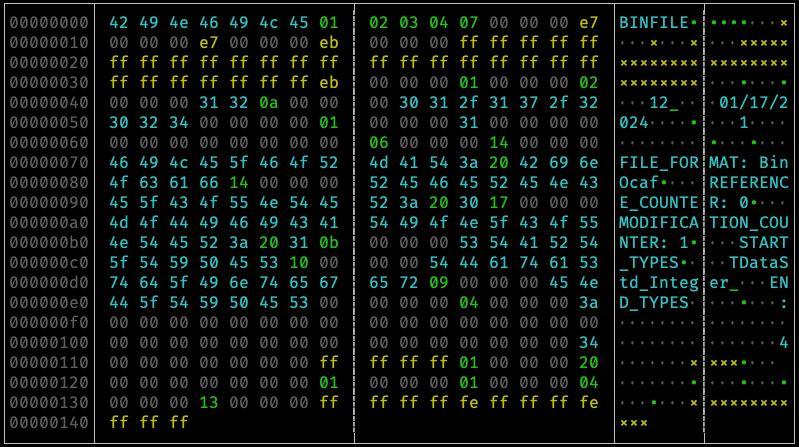
\includegraphics[width=.9\linewidth]{./img/binocaf-binary-content.png}
\end{center}

我们可以大致看到文档中包含了 creation-date file-format, reference-counter, modification-counter, \texttt{TDataStd\_Integer} 等一些信息。

在 \texttt{TDF\_Label} 中插入一个 \texttt{TopoDS\_Shape} 属性,可以使用 \texttt{XCAFDoc\_ShapeTool} 类或 \texttt{TNaming\_Builder} 类。 \texttt{XCAF} 模块提供了更高级的形状管理功能,而 \texttt{TNaming} 模块提供了更通用的命名和标识机制。
\subsection{相关的 OCCT 类}
\label{sec:orge9d0cc8}

\subsubsection{\texttt{TDocStd\_Application} class}
\label{sec:orgbe10c42}

类 \texttt{TDocStd\_Application} 用于创建、打开、保存、关闭和管理 OCAF 文档(\texttt{TDocStd\_Document}),支持多文档界面(MDI),允许同时处理多个文档。它是开发基于 OCAF 的应用程序的关键组件。

\begin{itemize}
\item \texttt{NewDocument(format: String, TDocStd\_Document\&)} 创建一个新的文档
\item \texttt{Open(path: String, TDocStd\_Document\&)} 打开磁盘上的一个文档
\item \texttt{Save(TDocStd\_Document\&)} 保存文档
\item \texttt{SaveAs(TDocStd\_Document\&, path: String)} 文档另存为
\item \texttt{Close(TDocStd\_Document\&)} 关闭文档
\end{itemize}
\subsubsection{\texttt{TDocStd\_Document} class}
\label{sec:org438a640}

类 \texttt{TDocStd\_Document} 代表一个 OCAF 文档,用于存储和管理复杂的工程数据。它包含一个或多个层次化的数据结构(通过 \texttt{TDF\_Label} 组织)。OCAF 文档支持事务处理机制,提供了 Undo/Redo 接口;支持文档的保存和加载。

\begin{itemize}
\item \texttt{IsSaved()} 检查文档是否已保存
\item \texttt{IsEmpty()} 检查文档是否为空,即 main label 是否包含 attributes
\item \texttt{NewCommand()} 启动一个新的事务或命令
\item \texttt{CommitCommand()} 提交当前事务,使其更改称为文档的一部分
\item \texttt{Undo()}, \texttt{Redo()} 撤销或重做最近的事务
\item \texttt{GetUndoLimit()}, \texttt{SetUndoLimit(int)} 获取和设置撤销操作的限制
\item \texttt{IsChanged()} 检查文档子上次保存后是否被修改
\item \texttt{SetModified(TDF\_Label\&)} 标记一个 label 为 modified,文档变为 UnValid 状态
\item \texttt{Recompute()} 重新计算,传播 modification 的影响
\item \texttt{IsValid()} 检查文档修改后,是否重新计算了
\item \texttt{Main()} 获取文档的 main label
\item \texttt{DumpJson(OStream\&)} 打印文档内容,用于调试 (文档中存在,但代码里不能使用)
\end{itemize}
\subsubsection{\texttt{TDF\_Label} class}
\label{sec:org10267a2}

类 \texttt{TDF\_Label} 代表文档 (\texttt{TDoc\_Std\_Document}) 中的一个数据节点,可以包含多个子节点 (\texttt{TDF\_Label}) 和与之关联的属性 (\texttt{TDF\_Attribute})。属性包含了各种拓扑形状,颜色,元数据等。它是 OCAF 中一种很基本的数据类型,用于组织和存储层次化的数据结构。

\begin{itemize}
\item \texttt{IsNull()} 检查标签是否为空。*注意*:只要标签不在 Document 中就为空,挺奇怪的。
\item \texttt{FindChild(Int tag, Bool create=True)} 查找或创建子 label
\item \texttt{NewChild()} 创建一个新的子 label,其 tag 自动生成
\item \texttt{HasChild()} 检查是否包含子 labels
\item \texttt{NbChildren()} 获取子 labels 的数量
\item \texttt{Father()} 获取当前 label 的父 label
\item \texttt{Tag()} 获取当前 label 的 Tag ID
\item \texttt{Root()} 获取文档的根标签。(这个接口感觉更应该放在 Document 中)
\item \texttt{Depth()} 获取 label 在文档层次结构中的深度
\item \texttt{HasAttribute()} 检查标签是否包含至少一个属性
\item \texttt{FindAttribute(GUID\&, TDF\_Attribute\&)} 根据 ID 查找属性
\item \texttt{AddAttribute(TDF\_Attribute\&)} 添加一个新的属性
\item \texttt{Dump(\&OStream)} 打印标签内容,用于调试 (文档中存在,但代码里不能使用)
\end{itemize}
\subsubsection{\texttt{TDataStd\_Integer} class}
\label{sec:orga4fd1a6}

类 \texttt{TDataStd\_Integer} 用于定义一个整数 attribute, 继承自 \texttt{TDF\_Attribute}, 是 \texttt{Standard\_Integer} 类型的封装。

\begin{itemize}
\item \texttt{Set(TDF\_Label\&, Standard\_Integer)} 静态函数,查找或创建一个整数属性,并设置其值为传入的参数。
\item \texttt{Get()}, \texttt{Set(Standard\_Integer)} 获取和设置内在的整数值 (不知道怎么用)
\end{itemize}
\subsubsection{\texttt{BinDrivers} class}
\label{sec:org751a0ff}

这个类只包含了三个静态函数,感觉像是个工具类。

\begin{itemize}
\item \texttt{DefineFormat(TDocStd\_Application\&)} 设置格式为 ``BinOcaf'',并为 app 注册读写驱动。
\end{itemize}
\subsection{几何形状的添加方式}
\label{sec:org477ea08}

前面的例子中,我们通过 \texttt{TDataStd\_Integer::Set(label, 123)} 语句往 \texttt{label} 中添加了一个整数属性。在各种属性中,最重要的是 \texttt{TopoDS\_Shape} 属性,但是 \texttt{TopoDS\_Shape} 类无法通过类似 \texttt{Set} 的静态函数进行添加。往 \texttt{TDF\_Label} 中添加 \texttt{TopoDS\_Shape} 属性的方式主要有两种: \texttt{TNaming\_Builder} 类和 \texttt{XCAFDoc\_ShapeTool} 类。 \texttt{TNaming} 模块提供了更通用的命名和标识机制; \texttt{XCAF} 模块提供了更高级的形状管理功能。

下面是使用 \texttt{TNaming\_Builder} 类添加 Shape 属性的代码示例:

\begin{minted}[]{cpp}
TDF_Label label;
TopoDS_Shape shape;

// 创建一个 TNaming_Builder
TNaming_Builder builder(label);
// 为 TopoDS_Shape 创建一个命名
builder.Generated(shape);
\end{minted}

下面是使用 \texttt{XCAFDoc\_ShapeTool} 类添加 Shape 属性的代码示例:

\begin{minted}[]{cpp}
TDF_Label label;
TopoDS_Shape shape;

// 获取 XCAFDoc_ShapeTool
Handle(XCAFDoc_ShapeTool) shapetool =
  XCAFDoc_DocumentTool::ShapeTool(label);
// 插入 TopoDS_Shape
TDF_Label label = shapetool->NewShape();
shapetool->SetShape(label, shape);
\end{minted}
\subsubsection{\texttt{TNaming\_Builder} class}
\label{sec:org81ee308}

\texttt{TNaming\_Builder} 类是在 OCAF 文档中创建和维护拓扑形状属性的工具类。其构造函数根据给定的标签创建一个空的 \texttt{TNaming\_NamedShape} 属性。它允许在该 NamedShape 中添加具有指定 evolution type 的 ``旧形状'' 和 ``新形状'' 对。

\begin{itemize}
\item \texttt{TNaming\_Builder(const TDF\_Label)} 构造函数的参数为要附加命名形状的 Label
\item \texttt{Generated(const TopoDS\_Shape\&)} 为给定的 Shape 创建一个 NamedShape, 并存储在关联的 Label 中。通常用于表示形状的创建或导入。
\item \texttt{Modify(const TopoDS\_Shape\& oldS, const TopoDS\_Shape\& newS)} 将 \texttt{oldS} 修改为 \texttt{newS}
\item \texttt{Delete(const TopoDS\_Shape\& S)} 将形状 \texttt{S} 从 label 中删除
\end{itemize}
\subsubsection{\texttt{XCAFDoc\_DocumentTool} class}
\label{sec:org9b5d819}

\texttt{XCAFDoc\_DocumentTool} 提供了一套工具和接口,用于在 OCAF 文档中处理和管理扩展的 CAD 数据,包括装配结构、颜色、层、材料等。

\begin{itemize}
\item \texttt{IsXCAFDocument(const Handle<TDocStd\_Document>\&)} 检查给定文档是否为 XCAF 文档。
\item \texttt{ShapeTool(const TDF\_Label\&)} 在参数 label 下的子标签 \texttt{DocLabel} 下获取或创建一个 \texttt{ShapeTool} 属性。
\item 类似地还有 \texttt{ColorTool()}, \texttt{MaterialTool()}, \texttt{ViewTool()}, \texttt{LayerTool()} 等方法。
\end{itemize}
\subsubsection{\texttt{XCAFDoc\_ShapeTool} class}
\label{sec:org7886da5}

\texttt{XCAFDoc\_ShapeTool} 类提供了一套工具,用于管理 XCAF 文档中的几何形状和装配结构。它支持装配结构的创建、管理和遍历,包括装配体、子装配体和零件。

\begin{itemize}
\item \texttt{NewShape()} 创建一个新的空 top-level Shape
\item \texttt{AddShape(const TopoDS\_Shape\&)} 想文档中添加一个现有形状
\item \texttt{SetShape(const TDF\_Label\&, const TopoDS\_Shape\&)} 设置标签与特定形状的关联。
\item \texttt{GetShapes()} 获取文档中的所有 top-level shapes
\item \texttt{AddComponent()} 将形状作为组件添加到装配体中,如有必要,为组件创建一个额外的顶层形状,并返回组件的标签
\item \texttt{GetComponents()} 获取装配体中的所有组件
\end{itemize}
\section{实现自定义 Labels\hfill{}\textsc{ATTACH}}
\label{sec:orga55a03b}
\subsection{Overview}
\label{sec:orgfd66e33}

OCAF 框架的 TDataStd package 为我们定义了很多基础的 \texttt{TDF\_Attribute} 类型,通过组织这些 attribute types (如 Integer, Real, String), 我们可以在 TDocStd\textsubscript{Document} 中创建所需的模型工件实例。但是这样的构建过程以及后续的访问和修改过程会变得非常琐碎啰嗦,因为我们需要逐级地访问深层的标签或属性。

类似于 DataBase 中的 data scheme,我们可以为 OCAF Document 中的工件实例,创建一些工件类型属性,它们比基础属性更加抽象,更贴近业务需求;并在创建的工件类型中定义一些贴近业务的访问与修改接口。最后当我们需要在 Document 中添加一个新的工件实例时,只需要调用工件类型的构造函数即可。

\begin{center}
\includegraphics[width=10cm]{/Users/chenchen/org/.attach/04/03220e-b530-4847-b0d0-ae2b31e8384f/_20240123_135714custom-labels.png}
\end{center}

上图是一个 Document 样例,在 root label 下有两个 main labels, \texttt{Parts} 和 \texttt{Meshes}, 它们分别表示几何模型和网格模型。然后在几何模型 \texttt{Parts} 下,我们可以根据模型的构成分成一些模型组件 \texttt{Part}, 每个模型组件具有独立的 Name, Shape, Color 等属性,同时它还会具有一些 \texttt{Feature} labels,用来包含 Shape 的 Face indices, Edge indices, Vertex indices 等信息。

在另一个 main label \texttt{Meshes} 下,包含了几何模型的网格数据。它的 sub-label 为 \texttt{Mesh} label。 \texttt{Mesh} 类型会包含网格数据 triangulation, 以及一些其他数据,如 reference,用于指向对应的几何 Part。这样当几何 Part 发生变化时,Mesh label 可以做相应的更新。

从上面的介绍,这个 app 中可以抽象出 3 个业务数据类型: \texttt{Part}, \texttt{Feature}, \texttt{Mesh} 。这三个数据类型,在业务上也是比较抽象的,后续可能会衍生一些更具体的类型。所以这里将它们定义为抽象接口,即 \texttt{IPart}, \texttt{IFeature}, \texttt{IMesh} 。
\subsection{\texttt{IPart} class}
\label{sec:org331ace5}

\subsubsection{\texttt{IPart} class 的定义}
\label{sec:org1676d55}

下面是 \texttt{IPart} 的实现代码

\begin{minted}[]{cpp}
class IPart {
public:
  IPart(const TDF_Label& label): m_root(label) {
    TDataStd_Name::Set(label, "Part");
  }

  void SetShape(const TopoDS_Shape& shape) {
    TNaming_Builder builder(m_root);
    builder.Generated(shape);
  }

  TopoDS_Shape GetShape() const {
    Handle(TNaming_NamedShape) attr;
    if (!m_root.FindAttribute(TNaming_NamedShape::GetID(), attr))
    {
      return TopoDS_Shape();
    }
    return attr->Get();
  }

  void SetColor(const unsigned r,
                const unsigned g,
                const unsigned b) {
    int icolor = (r << 16) | (g << 8) | b;
    TDataStd_Integer::Set(m_root, icolor);
  }

  bool GetColor(unsigned& r, unsigned& g, unsigned& b) {
    Handle(TDataStd_Integer) attr;
    if (!m_root.FindAttribute(TDataStd_Integer::GetID(), attr))
    {
      return false;
    }
    const int icolor = attr->Get();
    r = (icolor >> 16) & 0xFF;
    g = (icolor >>  8) & 0xFF;
    b = icolor & 0xFF;
    return true;
  }

private:
  TDF_Label m_root;
}
\end{minted}

\begin{itemize}
\item 上面的构造函数,传入一个 label 参数,表示对应的 Part label
\item 然后 \texttt{SetShape} 和 \texttt{GetShape} 方法用来设置和获取 Part 的 Shape 属性
\begin{itemize}
\item Shape attribute 和其他比较基础的 attribute 类型不太一样,因为我们需要记录 Shape 的历史演化版本,用于 Undo/Redo 功能。所以不能像其他基础属性一样,通过 Set 的方式直接存储到 Label 中,而是需要放到一个 \texttt{TNaming\_NamedShape} 中,然后在存储在对应的 Label 中。 \texttt{TNaming\_NamedShape} 提供了新旧版本的功能。
\item \texttt{TNaming\_Builder} 的构造函数根据给定的 label 创建一个空的 \texttt{TNaming\_NamedShape} 属性, 然后 \texttt{Generated} 方法将参数 \texttt{TopoDS\_Shape} 实例存储到 NamedShape 属性中。
\end{itemize}
\item 同样地, \texttt{SetColor}  和 \texttt{GetColor} 方法用于设置和获取 Part 的 Color 属性
\begin{itemize}
\item 这里 \texttt{Color} 使用一个 Integer 来存储。通过位操作运算来设置和获取 Color 的值
\end{itemize}
\end{itemize}

注意: 上面的 \texttt{TNaming} 中的 \texttt{T} 是 Topological 的缩写;而在另一些情况下,如 \texttt{TDocStd} 中, \texttt{T} 则是 Transient 的缩写。这有时会让人困惑。
\subsubsection{使用 \texttt{IFeature} 类}
\label{sec:orgb40365c}

下面是在 Application 的文档中创建 Part label 的示例代码:

\begin{minted}[]{cpp}
TDF_Label parts_label = doc->Main();

IPart part1(TDF_TagSource::NewChild(parts_label));
IPart part2(TDF_TagSource::NewChild(parts_label));
IPart part3(TDF_TagSource::NewChild(parts_label));

BRepPrimAPI_MakeBox box(1, 2, 3);
part2.SetShape(box.Shape());
part2.SetColor(255, 0, 0);
\end{minted}

\begin{itemize}
\item 上面的代码在 main label \texttt{parts\_label} 下创建了三个 part labels: \texttt{part1}, \texttt{part2}, \texttt{part3}.
\begin{itemize}
\item 在创建 \texttt{IPart} 实例时,首先通过 \texttt{TDF\_TagSource::NewChild} 函数在 \texttt{parts\_label} 下创建 child labels, 并自动分配 Tag。
\item 然后将新创建的 child label 传给 \texttt{IPart} 构造函数, 来创建 \texttt{IPart} 实例。
\item 注意这里 \texttt{IPart} 不包含 \texttt{TDF\_Label} 而是引用它。
\end{itemize}
\item 然后为 \texttt{part2} 设置了 Shape 和 Color 属性。
\end{itemize}
\subsection{\texttt{IFeature} class}
\label{sec:org25a32ce}

\subsubsection{\texttt{IFeature} class 的定义}
\label{sec:org02f3d54}

下面是 \texttt{IFeature} class 的实现:

\begin{minted}[]{cpp}
class IFeature {
  public:
  IFeature(const TDF_Label& label): m_root(label) {
  }

  void SetFaces(const TColStd_PackedMapOfInteger& fids) {
    Handle(TDataStd_IntPackedMap) attr =
      TDataStd_IntPackedMap::Set(m_root);
    attr->ChangeMap(fids);
  }

  private:
  TDF_Label m_root;
}
\end{minted}

\begin{itemize}
\item 和 \texttt{IPart} 类似,构造函数传入的参数为 feature 对应的 label。
\item 方法 \texttt{SetFaces} 在 feature label 中添加一个 face-id 作为其属性
\end{itemize}
\subsubsection{\texttt{TDataStd\_IntPackedMap} class}
\label{sec:org2256694}

\texttt{TDataStd\_IntPackedMap} 类用于在 OCAF 文档中存储和管理一组整数值的集合(如 ID、索引或其他整数标识符)。它可以被附加到 \texttt{TDF\_Label} 上,用于表示和管理与该标签相关联的一组整数。

\begin{itemize}
\item \texttt{ChangeMap(const TColStd\_PackedMapOfInteger\&)} 改变内部存储的 integer map。
\item \texttt{IsEmpty()} 检查集合是否为空
\item \texttt{Extend()} 获取集合中元素的数量
\item \texttt{Add(const Standard\_Integer)} 向集合中添加一个整数值
\item \texttt{Remove(const Standard\_Integer)} 从集合中移除一个整数值
\item \texttt{Contains(const Standard\_Integer)} 检查集合中是否包含指定的整数值
\item \texttt{Clear()} 清空集合中的所有元素
\end{itemize}
\subsubsection{使用 \texttt{IFeature} 类}
\label{sec:org156f118}

\begin{minted}[]{cpp}
class IPart {
  //...
  IFeature CreateFeature(const TColStd_PackedMapOfInteger& fids) {
    TDF_Label feat_root_lab = TDF_TagSource::NewChild(m_root);
    IFeature feature(feat_root_lab);
    feature.SetFaces(fids);
    return feature;
  }

  void GetFeatures(std::vector<IFeature>& features) {
    for (TDF_ChildIterator cit(m_root); cit.More(); cit.Next()) {
      features.push_back(IFeature(cit.Value()));
    }
  }
}

TColStd_PackedMapOfInteger fids1, fids2;
fids1.Add(1);
fids1.Add(2);
fids1.Add(3);
fids2.Add(3);
fids2.Add(4);
fids2.Add(5);
part3.CreateFeature(fids1);
part3.CreateFeature(fids2);

std::vector<IFeature> part3_features;
part3.GetFeatures(part3_features);
\end{minted}

\begin{itemize}
\item 在 \texttt{IPart} 类中,我们为其定义了创建和获取 feature 子标签的方法。
\begin{itemize}
\item \texttt{CreateFeature} 传入的参数为 Part 的 face-ids, 即所有的面标识符
\item \texttt{GetFeatures} 中通过 \texttt{TDF\_ChildIterator} 迭代器来遍历 part label 下的所有 feature labels。
\end{itemize}
\item main 函数中, 创建了两个整数集合,作为 face-ids,然后在 \texttt{part3} 下创建两个 feature 标签。
\item 最后通过 \texttt{GetFeatures} 方法获取所有的 features, 放在一个 vector 中。
\end{itemize}
\subsubsection{\texttt{TDF\_ChildIterator} class}
\label{sec:org702e493}

\texttt{TDF\_ChildIterator} 类通过提供一种简单而有效的方法来遍历 \texttt{TDF\_Label} 的子标签,使得开发者方便地访问和操作 OCAF 文档中的层次化数据。

\begin{itemize}
\item \texttt{TDF\_ChildIterator(const TDF\_Label\&, const Standard\_Boolean)} 构造函数,可以接受一个 label 和一个 bool 值。bool 参数用于指定是仅遍历第一层子标签,还是遍历所有层次的子标签(深度优先)。
\item \texttt{More()} 检查是否还有更多的子标签可以遍历
\item \texttt{Next()} 移动到下一个子标签
\item \texttt{Value()} 获取当前子标签
\end{itemize}
\subsection{\texttt{IMesh} 类}
\label{sec:org94ec631}

\subsubsection{\texttt{IMesh} 类的定义}
\label{sec:orgc97f9fb}

\begin{minted}[]{cpp}
class IMesh {
  public:
  IMesh(const TDF_Label& label): m_root(label) {
  }

  void Create(const IPart& part) {
    TopoDS_Shape part_shape = part.GetShape();
    Handle(Poly_Triangulation) mesh;
    for (TopExp_Explorer exp(part_shape, TopAbs_FACE);
         exp.More();
         exp.Next()) {
      const TopoDS_Face& face = TopoDS::Face(exp.Current());
      TopLoc_Location loc;
      mesh = BRep_Tool::Triangulation(face, loc);
      break;
    }
    if (mesh.IsNull()) {
      return;
    }
    TDataXtd_Triangulation::Set(m_root, mesh);

    TDF_Reference::Set(m_root, part.GetLabel());
  }

  private:
  TDF_Label m_root;
}
\end{minted}

\begin{itemize}
\item Mesh 在文档中也是一个 label。其构造函数和 \texttt{IPart}, \texttt{IFeature} 类似。
\item \texttt{Creat} 方法中, 通过 \texttt{TopExp\_Explorer} 遍历 part shape 的所有 Face 元素。
\begin{itemize}
\item \texttt{TopoDS::Face} 函数将当前拓扑元素从类型 \texttt{TopoDS\_Shape} 转换为 \texttt{TopoDS\_Face}
\end{itemize}
\end{itemize}
\subsubsection{\texttt{TopExp\_Explorer} 类}
\label{sec:org3d382f8}

\texttt{TopExp\_Explorer} 类提供了一种高效的方式来遍历和访问 \texttt{TopoDS\_Shape} 中的拓扑元素,使得开发者可以方便地对 Shape 内部结构的深入了解和控制。

\begin{itemize}
\item \texttt{TopExp\_Explorer(const TopoDS\_Shape\&, const TopAbs\_ShapeEnum to\_find, const TopAbs\_ShapeEnum to\_avoid)} 在构造函数的参数中,可以指定要遍历的 Shape, 遍历的元素类型(如 \texttt{TopAbs\_VERTEX}, \texttt{TopAbs\_EDGE} 等)。其中 \texttt{to\_find} 参数为要遍历的元素类型, \texttt{to\_avoid} 参数为忽略的元素类型, 默认为 \texttt{TopAbs\_SHAPE}
\item \texttt{Current()} 获取当前遍历到的元素
\item \texttt{Depth()} 返回当前遍历的深度
\end{itemize}
\subsubsection{\texttt{TopLoc\_Location} 类}
\label{sec:org62568df}

\texttt{TopLoc\_Location} 类用于定义几何形状在三维空间中的位置和方向,可以表示平移、旋转和缩放等变换,以及这些变换的组合。 \texttt{TopLoc\_Location} 通常与 \texttt{TopoDS\_Shape} 对象结合使用,以定义形状在空间中的放置。

\begin{itemize}
\item \texttt{TopLoc\_Location(const gp\_Trsf\&)} 基于给定的变换矩阵创建一个默认的位置
\item \texttt{IsIdentity()} 检查位置是否为恒等变换
\item \texttt{Transformation()} 获取与位置相关的变换矩阵(\texttt{gp\_Trsf})
\item \texttt{Inverted()} 获取位置的逆变换
\item \texttt{Multiplied(const TopLoc\_Location\&)} 将当前位置与另一个位置相乘,得到复合变换。
\item \texttt{FirstDatum()} 和 \texttt{FirstPower()} 在位置表示为一系列变换的序列时,获取第一个变换及其次数。
\end{itemize}
\subsubsection{\texttt{BRep\_Tool} 类}
\label{sec:org90810a4}

\texttt{BRep\_Tool} 是一个工具类,提供对 \texttt{BRep} 形状 (如 \texttt{TopoDS\_Vertex}, \texttt{TopoDS\_Edge} 等) 的查询和访问。它是 OCCT 中用于处理几何形状的核心工具之一,尤其在 \texttt{BRep} 建模中。

\begin{itemize}
\item \texttt{Triangulation(const TopoDS\_Face\&, TopLoc\_Location\&)} 该静态函数用于从 \texttt{TopoDS\_Face} 对象中提取三角化的网格数据,该 face 需要已经被三角化。
\begin{itemize}
\item 三角化是将 CAD 模型中的曲面近似表示为三角形网格的过程。
\item 它返回一个 \texttt{Poly\_Triangulation} 对象。
\item \texttt{Poly\_Triangulation} 类用于表示三角化的网格数据,存储了曲面三角化的结果,包括顶点坐标、三角形索引,以及可选的法线和纹理坐标,通常用于可视化和几何分析。
\end{itemize}
\end{itemize}
\subsubsection{\texttt{TDataXtd\_Triangulation}, \texttt{Poly\_Triangulation} 类}
\label{sec:org52aaaef}

\texttt{TDataXtd\_Triangulation} 类是 \texttt{TDF\_Attribute} 的子类型,可以理解为对 \texttt{Poly\_Triangulation} 的简单封装,主要接口和功能一致。

\texttt{Poly\_Triangulation} 类用于存储三角化后的网格数据,使得开发者可以对几何形状进行有效的可视化和处理。它封装了三角化曲面及其他的几何形状数据,包括顶点坐标和三角形的拓扑结构。

\begin{itemize}
\item \texttt{NbNodes()} 获取三角网格的顶点数量
\item \texttt{NbTriangles()} 获取三角网格中三角形的数量
\item \texttt{InternalNodes()} 返回所有顶点的内部数组
\item \texttt{Triangles()} 返回包含所有三角形索引的数组。每个三角形由三个顶点索引组成。
\item \texttt{InternalUVNodes()} 返回包含 UV 纹理坐标的数组。
\end{itemize}
\subsubsection{\texttt{TDF\_Reference} 类}
\label{sec:org1cfae96}

\texttt{TDF\_Reference} 类提供了一种方式来在 OCAF 文档的一个 label 中存储对另一个 label 的引用,来增强 OCAF 的数据组织和管理能力。它用于表示复杂的数据关系,如链接到共享数据、创建装配结构的引用等。

\begin{itemize}
\item \texttt{Set(const TDF\_Label\& source, const TDF\_Label\& target)} 在 source 标签上创建一个对 target 标签的引用。
\item \texttt{Get()} 获取当前引用所指向的标签。
\end{itemize}
\section{实现自定义的 Attribute}
\label{sec:org4f3a8b2}




\section{OCAF 实现参数化设计}
\label{sec:org7ac6a4a}

下面的代码基于 OCAF 实现了一个参数化设计程序。
\section{基于 IVtk Package 实现一个 VTK 模型查看器}
\label{sec:orga2f4a0c}

这个例子使用开源的 VTK 包作为 OCCT 的 3D 渲染前端。OCCT 提供了一个 \texttt{IVtk} package,它为 OCCT 的基础类型 \texttt{TopoDS} 和 VTK 的基础类型 \texttt{vtkPolyData} 提供了一个适配器。
\subsection{程序代码}
\label{sec:org56c35c9}

下面是项目的 \texttt{CMakeLists.txt} 文件内容:

\begin{minted}[]{cmake}
cmake_minimum_required(VERSION 3.10)
project(demo)

find_package(OpenCASCADE REQUIRED)
find_package(VTK REQUIRED)

include_directories(
  ${OpenCASCADE_INCLUDE_DIR}
  ${VTK_INCLUDE_DIR}
)

set(SOURCES main.cpp)
add_executable(${CMAKE_PROJECT_NAME} ${SOURCES})

target_link_libraries(${CMAKE_PROJECT_NAME}
  ${OpenCASCADE_LIBRARIES}
  ${VTK_LIBRARIES}
)
\end{minted}

下面是示例的源代码:

\begin{minted}[]{cpp}
#include <BRepPrimAPI_MakeBox.hxx>
#include <IVtkTools_ShapeDataSource.hxx>

#include <vtkAutoInit.h>
#include <vtkRenderer.h>
#include <vtkRenderWindow.h>
#include <vtkRenderWindowInteractor.h>
#include <vtkInteractorStyleTrackballCamera.h>
#include <vtkPolyDataMapper.h>

VTK_MODULE_INIT(vtkRenderingOpenGL2)
VTK_MODULE_INIT(vtkInteractionStyle)

int main() {
  /// Build a simple OCCT model
  BRepPrimAPI_MakeBox box(1., 2., 3.);
  const auto& shape = box.Shape();

  /// Setup VTK Render
  vtkNew<vtkRenderWindow> renwin;

  vtkNew<vtkRenderer> ren;
  renwin->AddRenderer(ren);

  vtkNew<vtkRenderWindowInteractor> iren;
  vtkNew<vtkInteractorStyleTrackballCamera> istyle;
  iren->SetRenderWindow(renwin);
  iren->SetInteractorStyle(istyle);

  /// Bridge OCCT and VTK with IVtk package
  // TopoDS_Shape -> vtkPolyData -> <filters> -> mapper -> actor
  vtkNew<IVtkTools_ShapeDataSource> occSource;
  occSource->SetShape(new IVtkOCC_Shape(shape));

  vtkNew<vtkPolyDataMapper> mapper;
  mapper->SetInputConnection(occSource->GetOutputPort());

  vtkNew<vtkActor> actor;
  actor->SetMapper(mapper);
  ren->AddActor(actor);

  // Start the render window app
  renwin->Render();
  iren->Start();

  return 0;
}
\end{minted}

下面是程序运行后,模型的显示效果:

\begin{center}
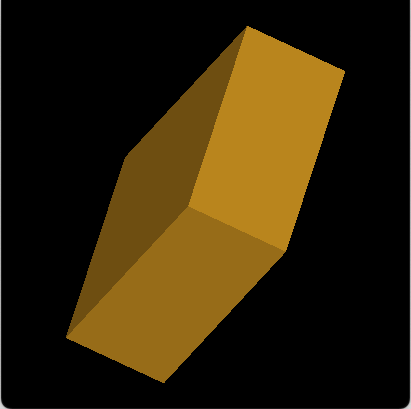
\includegraphics[width=.9\linewidth]{./img/occt-vtk-viewer.png}
\end{center}
\subsection{相关的类}
\label{sec:orgee030c1}

\subsubsection{\texttt{IVtkTools\_ShapeDataSource} class}
\label{sec:org6715d3a}

这个类用于将 OCCT 中的 BRep 拓扑结构数据 (如 \texttt{TopoDS\_Shape}) 转换为 VTK 的数据结构 (如 \texttt{vtkPolyData}, \texttt{vtkUnstructuredGrid}),从而能够在 VTK 环境中进行可视化和处理。

\begin{itemize}
\item \texttt{SetShape(IVtkOCC\_Shape::Handle \&occShape)} 设置要转换的源 OCCT 形状对象
\item \texttt{GetShape()} 获取当前设置的源 OCCT 形状对象。
\item \texttt{GetOutputPort()} 方法来自于其所继承的 \texttt{vtkPolyDataAlgrithm} 类,用于获取与给定输出端口对应的代理对象。代理对象可以传递给其他算法的 \texttt{SetInputConnection}, \texttt{AddInputConnection} 等方法,以修改管道连接。
\end{itemize}
\subsubsection{\texttt{IVtkOCC\_Shape} class}
\label{sec:orgbb3a6b7}

这个类用于将 OCCT 中的形状类型 (\texttt{TopoDS\_Shape}) 转换为 VTK 数据类型,以便在 VTK 中可以直接可视化和操作 OCCT 中的形状对象。

\begin{itemize}
\item \texttt{GetShape() -> TopoDS\_Shape\&} 获取当前设置的 OCCT 形状。
\end{itemize}
\end{document}
